\chapter{Product Backlog}
Per una visione generale del progetto, di seguito vengono inserite le immagini del \href{https://github.com/orgs/ISIQuiz/projects/3/views/2}{product backlog by progress}. In particolare, queste indicano la chiusura delle varie user story all'interno degli sprint anche se esse sono state iniziate precedentemente. Ad esempio, l'interfaccia grafica è stata iniziata nello sprint 8, ma conclusa solo nel 10. Poiché ad una user-story non possono essere assegnati più sprint, essa appare solo nel suddetto Sprint Backlog, mentre i suoi refinement sono presenti anche negli altri.

\begin{figure}[H]
    \centering
    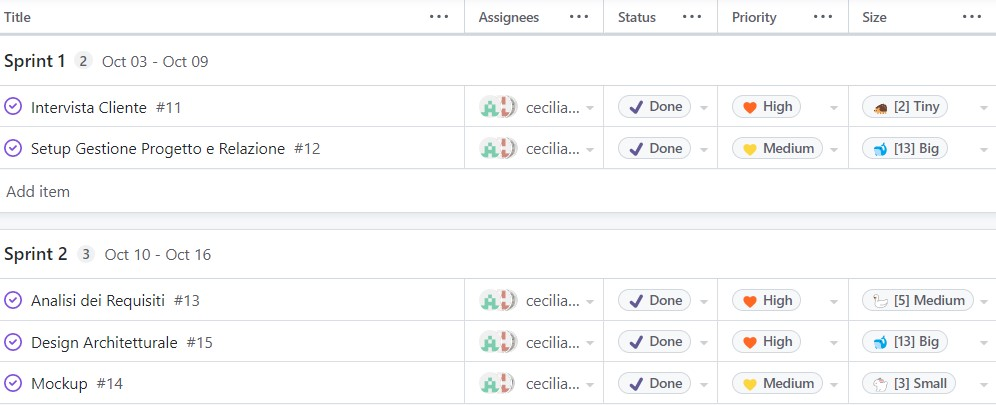
\includegraphics[width=\textwidth]{process/Img/sprint1_2.jpg}
    \label{fig:Sprint1_2}
\end{figure}
\begin{figure}[H]
    \centering
    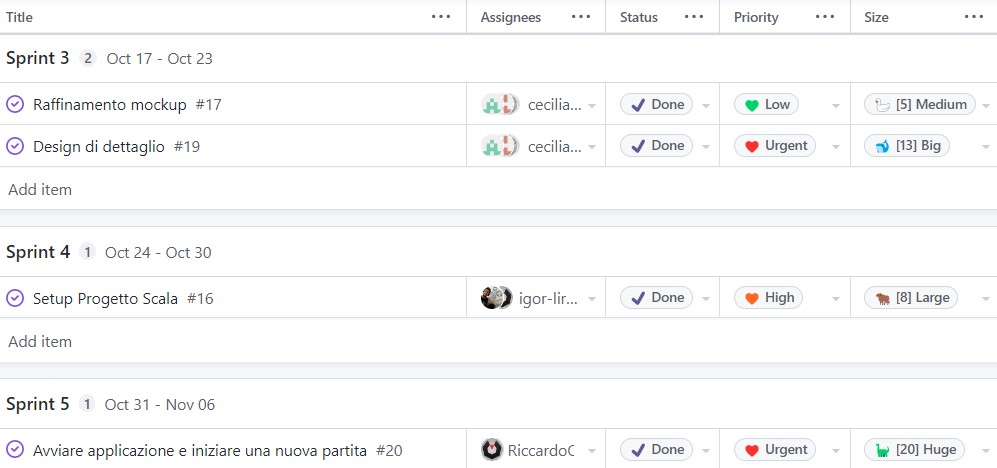
\includegraphics[width=\textwidth]{process/Img/sprint3_4_5.jpg}
    \label{fig:Sprint3_4_5}
\end{figure}
\begin{figure}[H]
    \centering
    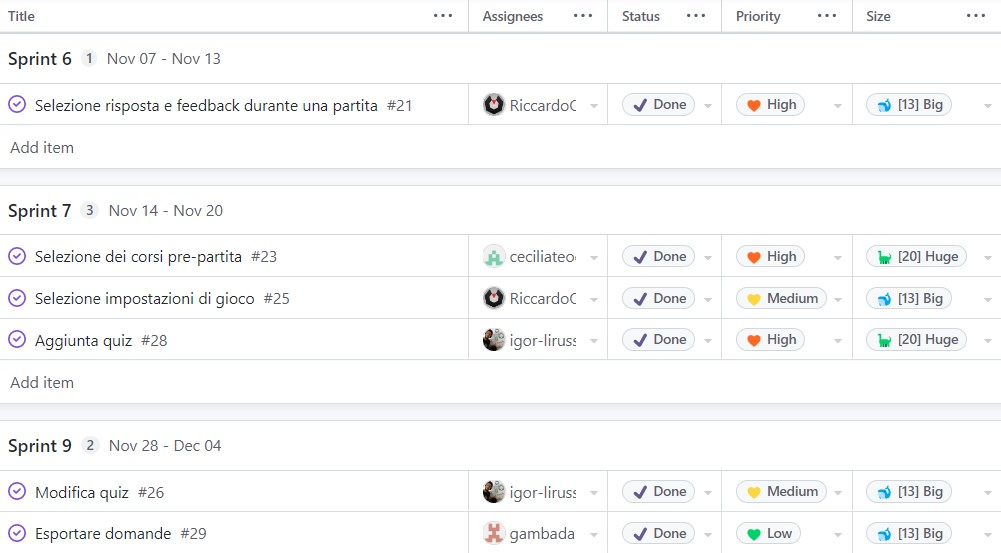
\includegraphics[width=\textwidth]{process/Img/sprint6_7_9.jpg}
    \label{fig:Sprint6_7_9}
\end{figure}
\begin{figure}[H]
    \centering
    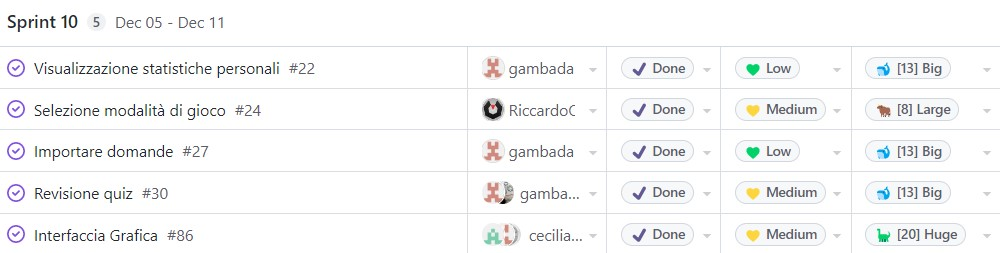
\includegraphics[width=\textwidth]{process/Img/sprint10.jpg}
    \label{fig:Sprint10}
\end{figure}

Nel capitolo finale \ref{chap:final-stats} sono invece inseriti dei grafici relativi al processo di sviluppo.